\documentclass[11pt,a4paper]{article}
\usepackage[margin=18mm,top=22mm,bottom=20mm]{geometry}
\usepackage{fontspec}\setmainfont{Latin Modern Roman}
\usepackage{amsmath,amssymb,tikz,graphicx,fancyhdr,array,needspace}
\usetikzlibrary{patterns,arrows.meta,decorations.pathmorphing,calc}
\setlength{\headheight}{14pt}
\usetikzlibrary{arrows.meta}
\pagestyle{fancy}\fancyhf{}\renewcommand{\headrulewidth}{0.4pt}
\fancyhead[L]{\textbf{M-01}}\fancyhead[C]{\itshape Fizika (OliyFizika.uz mock test)}\fancyhead[R]{\textbf{Mock №1}}
\fancyfoot[C]{\thepage}
\setlength{\parindent}{0pt}\setlength{\parskip}{3pt}
\newcommand{\opt}[2]{\hspace*{4mm}#1)\ #2\par}
\newcommand{\blank}{\rule{5cm}{0.4pt}}
\begin{document}

\begin{center}{\Large\textbf{FIZIKA}}\end{center}
\noindent\begin{minipage}{\linewidth}
\textbf{1.}\ Poyezd 2 m/s tezlikda ketayotgan piyodani 15 s da quvib ötdi. 96 m li tunneldan esa 18 s da ötdi. Poyezdning uzunligi qançaga (m) teng?\par\smallskip
\opt{A}{100 m}
\opt{B}{200 m}
\opt{C}{250 m}
\opt{D}{300 m}
\end{minipage}\vspace{9pt}\par
\noindent\begin{minipage}{\linewidth}
\textbf{2.}\ Radiusi 1 cm bölgan temir şarni radiusi 3 cm ga yetgunça oltin ($\rho_{oltin}$ = 19300 kg/m$^{3}$) bilan qoplandi. Bu jarayonga qança (kg) oltin sarflanganini aniqlang. $\pi$ = 3\par\smallskip
\opt{A}{0,62}
\opt{B}{2}
\opt{C}{1,54}
\opt{D}{1}
\end{minipage}\vspace{9pt}\par
\noindent\begin{minipage}{\linewidth}
\textbf{3.}\ Har qanday avtotebranişlar tizimi..... kabi qismlardan iborat böladi.\par\smallskip
\opt{A}{tebraniş tizimi va elektron kalit}
\opt{B}{energiya manbai, tebraniş tizimi}
\opt{C}{energiya manbai, tebraniş tizimi va elektron kalit}
\opt{D}{energiya manbai, tebraniş tizimi, elektron kalit va töğirlagiç}
\end{minipage}\vspace{9pt}\par
\noindent\begin{minipage}{\linewidth}
\textbf{4.}\ Uç jism bir xil balandlikdan erkin tuşyapti. 1-jismning boşlanğiç tezligi yöq, 2 va 3-jismlarning boşlanğiç tezliklari gorizontal yönalgan ($v_2<v_3$). Ularning yerga tuşiş vaqtlarini taqqoslang.\par\smallskip
\opt{A}{$t_1<t_2<t_3$}
\opt{B}{$t_1=t_2=t_3$}
\opt{C}{$t_1>t_2>t_3$}
\opt{D}{$t_1<t_2=t_3$}
\end{minipage}\vspace{9pt}\par
\noindent\begin{minipage}{\linewidth}
\textbf{5.}\ Massasi $m$ bölgan çana balandligi $h$ bölgan tepalikdan sirpanib tuşdi va tekis yerda biror masofa ötib töxtadi. Çanani dastlabki vaziyatga qaytariş uçun qança iş bajariş kerak? Butun yöl davomida işqalaniş koeffitsiyenti bir xil.\par\smallskip
\opt{A}{2$mgh$}
\opt{B}{4$mgh$}
\opt{C}{3$mgh$}
\opt{D}{$mgh$}
\end{minipage}\vspace{9pt}\par
\noindent\begin{minipage}{\linewidth}
\textbf{6.}\ Jism 80 m öngga, keyin esa 30 m qarama-qarşi tomonga yuridi. Jismning köçisini (m) aniqlang.\par\smallskip
\opt{A}{50}
\opt{B}{25}
\opt{C}{75}
\opt{D}{100}
\end{minipage}\vspace{9pt}\par
\noindent\begin{minipage}{\linewidth}
\textbf{7.}\ Diametri 0,8 mm bölgan simning uzunligi 3,14 m ga teng. 64 N kuç ta’siri ostida sim 2 mm uzaydi. Simning Yung modulini toping (GPa).\par\smallskip
\opt{A}{300}
\opt{B}{150}
\opt{C}{100}
\opt{D}{200}
\end{minipage}\vspace{9pt}\par
\noindent\begin{minipage}{\linewidth}
\textbf{8.}\ Massasi 400 g bölgan jismning tezligi 10 m/s ga teng. Uning kinetik energiyasini (J) aniqlang.\par\smallskip
\opt{A}{2}
\opt{B}{10}
\opt{C}{30}
\opt{D}{20}
\end{minipage}\vspace{9pt}\par
\noindent\begin{minipage}{\linewidth}
\textbf{9.}\ Uzunligi 13 m va balandligi 5 m bölgan qiya tekislikda massasi 26 kg bölgan yuk yotibdi. Işqalaniş koeffitsiyenti 0,5 ga teng. Yukni yuqoriga çiqariş uçun tekislik böylab unga qanday kuç qöyiş lozim (N)? Tuşiriş uçunçi (N)? g=10 N/kg.\par\smallskip
\opt{A}{220; 20}
\opt{B}{200; 10}
\opt{C}{20; 10}
\opt{D}{5; 10}
\end{minipage}\vspace{9pt}\par
\noindent\begin{minipage}{\linewidth}
\textbf{10.}\ $m$ massali şarça $v$ tezlik bilan harakatlanib, huddi şunday tinç turgan şarçaga noelastik urildi va birgalikda harakatni davom ettirişdi. Töqnaşuvdan keyin sistema energiyasi neça marta kamayadi?\par\smallskip
\opt{A}{4 marta}
\opt{B}{2 marta}
\opt{C}{8 marta}
\opt{D}{3 marta}
\end{minipage}\vspace{9pt}\par
\noindent\begin{minipage}{\linewidth}
\textbf{11.}\ Şarqdan 100 km/h tezlikda şamol esmoqda. Tezligi 100 km/h bölgan vertolyot qanday kursni tanlasa, aniq şimoliy yönalişda uça oladi?\par\smallskip
\opt{A}{şimoli-şarqiy yönalişda, meridianga nisbatan 45$^\circ$ burçak ostida}
\opt{B}{şimoli-ğarbiy yönalişda, meridianga nisbatan 45$^\circ$ burçak ostida}
\opt{C}{şimoli-şarqiy yönalişda, meridianga nisbatan 60$^\circ$ burçak ostida}
\opt{D}{aniq şimoliy yönalişda uça olmaydi}
\end{minipage}\vspace{9pt}\par
\noindent\begin{minipage}{\linewidth}
\textbf{12.}\ Normal şaroitda har qanday gazning birlik hajmdagi molekulalar soni nimaga teng?\par\smallskip
\opt{A}{Avogadro soniga}
\opt{B}{Faradey soniga}
\opt{C}{Loşmidt soniga}
\opt{D}{Boltsman soniga}
\end{minipage}\vspace{9pt}\par
\noindent\begin{minipage}{\linewidth}
\textbf{13.}\ 1/3 qismi dissotsiatsiyalangan 64 g kislorodning modda miqdorini aniqlang (mol). M($O_2$)=32 g/mol.\par\smallskip
\opt{A}{0,5}
\opt{B}{1}
\opt{C}{2}
\opt{D}{8/3}
\end{minipage}\vspace{9pt}\par
\noindent\begin{minipage}{\linewidth}
\textbf{14.}\ Moddada har bir atom qöşni atom bilan elektron jufti orqali birikişi ..... boğlaniş deb ataladi.\par\smallskip
\opt{A}{ion}
\opt{B}{metall}
\opt{C}{kovalent}
\opt{D}{vodorod}
\end{minipage}\vspace{9pt}\par
\noindent\begin{minipage}{\linewidth}
\textbf{15.}\ Massasi 16 g bölgan geliyni ($M$=4 g/mol) 10 K ga izobarik qizdiriş uçun ketgan issiqlik miqdori bilan, massasi 10 g bölgan neon ($M$=20 g/mol) izotermik ravişda qança iş (J) bajaradi?\par\smallskip
\opt{A}{831}
\opt{B}{1163}
\opt{C}{416}
\opt{D}{499}
\end{minipage}\vspace{9pt}\par
\noindent\begin{minipage}{\linewidth}
\textbf{16.}\ Qarşilik kuçi 20 kN bölganda, 5 m/s tezlik bilan tekis harakatlanayotgan maşina motorining quvvati 400 kW bölsa, FIK neça foiz böladi?\par\smallskip
\opt{A}{50}
\opt{B}{40}
\opt{C}{25}
\opt{D}{30}
\end{minipage}\vspace{9pt}\par
\noindent\begin{minipage}{\linewidth}
\textbf{17.}\ 2 soat davom etgan elektrolizda katodda 14 g kumuş ajralib çiqdi. Elektroliz jarayoni yana 4 soat davom ettirilsa hammasi bölib qança (g) kumuş olinadi?\par\smallskip
\opt{A}{56}
\opt{B}{28}
\opt{C}{64}
\opt{D}{42}
\end{minipage}\vspace{9pt}\par
\noindent\begin{minipage}{\linewidth}
\textbf{18.}\ Qizuvçi simlari volframdan yasalgan ikki lampa özgarmas kuçlaniş manbayiga parallel ulanganida birinçi lampa ravşanroq yondi. Agar ular tarmoqqa ketma-ket ulansa, qanday yonadi?\par\smallskip
\opt{A}{ikkisi birdek yonadi}
\opt{B}{ikkinçisi ravşanroq yonadi}
\opt{C}{birinçisi ravşanroq yonadi}
\opt{D}{avval ikkinçisi, söngra birinçisi ravşanroq yonadi}
\end{minipage}\vspace{9pt}\par
\noindent\begin{minipage}{\linewidth}
\textbf{19.}\ Köndalang kesim yuzalari 1 cm$^{2}$ va 2 cm$^{2}$ bölgan ikkita bir xil uzunlikli simlar özaro yonma-yon birlaştirilib, 3 N kuç bilan çözildi. Simlarning mexanik kuçlanişini toping (kPa).\par\smallskip
\opt{A}{1}
\opt{B}{10}
\opt{C}{2}
\opt{D}{20}
\end{minipage}\vspace{9pt}\par
\noindent\begin{minipage}{\linewidth}
\textbf{20.}\ Qarşiligi 1 $\Omega$ bölgan ampermetrga 0,2 $\Omega$ qarşilik parallel ulansa, uning ölçaş çegarasi neça marta ortadi?\par\smallskip
\opt{A}{1}
\opt{B}{2}
\opt{C}{6}
\opt{D}{8}
\end{minipage}\vspace{9pt}\par
\noindent\begin{minipage}{\linewidth}
\textbf{21.}\ Özaro elektrostatik ta’sirlaşayotgan ikkita zaryadlangan şarçalar orasiga ma’lum bir qalinlikdagi dielektrik modda joylaştirilgan. Şarçalarning özaro ta’sirlaşiş kuçini toping (nN). $\varepsilon$=2.\par\smallskip
\noindent\hspace*{4mm}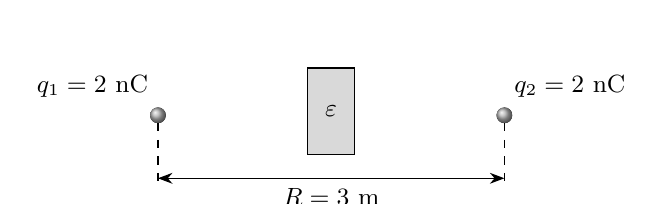
\begin{tikzpicture}[x=1cm,y=1cm,line width=0.5pt,>=Stealth,font=\small]
\fill[ball color=gray!60] (0,0) circle(0.1); \node[above left] at (0,0.1) {$q_1=2\ \mathrm{nC}$};
\fill[ball color=gray!60] (4.4,0) circle(0.1); \node[above right] at (4.4,0.1) {$q_2=2\ \mathrm{nC}$};
\draw[fill=gray!30] (1.9,-0.5) rectangle (2.5,0.6); \node at (2.2,0.05) {$\varepsilon$};
\draw[dashed] (0,-0.1)--(0,-0.9) (4.4,-0.1)--(4.4,-0.9); \draw[<->] (0,-0.8)--(4.4,-0.8); \node[below] at (2.2,-0.8) {$R=3\ \mathrm{m}$};
\end{tikzpicture}\par\smallskip
\opt{A}{2}
\opt{B}{4}
\opt{C}{8}
\opt{D}{12}
\end{minipage}\vspace{9pt}\par
\noindent\begin{minipage}{\linewidth}
\textbf{22.}\ Kabel har birining kesimi 0,6 mm$^{2}$ dan bölgan ikkita pölat toladan va har birining kesimi 0,85 mm$^{2}$ dan bölgan törtta mis toladan iborat. Tok kuçi 0,1 A bölganda kabelning har bir kilometridagi kuçlaniş tuşuvi qanday böladi (V)? $\rho$pöl =1,2$\cdot10^{-7}$ $\Omega$ $\cdot$ m, $\rho$mis =1,7$\cdot10^{-8}$ $\Omega$ $\cdot$ m.\par\smallskip
\opt{A}{0,16}
\opt{B}{0,9}
\opt{C}{0,48}
\opt{D}{20}
\end{minipage}\vspace{9pt}\par
\noindent\begin{minipage}{\linewidth}
\textbf{23.}\ Akkumulyatorning EYuK 12 V, töplagan zaryadi 30 A$\cdot$h. Akkumulyator qança energiya (kJ) bera oladi? Akkumulyator FIK ni 100 \% deb hisoblang.\par\smallskip
\opt{A}{1944}
\opt{B}{1728}
\opt{C}{1296}
\opt{D}{2376}
\end{minipage}\vspace{9pt}\par
\noindent\begin{minipage}{\linewidth}
\textbf{24.}\ Qarşiligi 2 $\Omega$ bölgan rezistor kuçlanişi $u = 4\sqrt{2}\cos(\dfrac{\pi}{8}t)$ [V] qonun böyiça özgaradigan özgaruvçan tok manbayiga ulandi. $t$=10 s paytdagi tokning oniy quvvatini (W) aniqlang.\par\smallskip
\opt{A}{8}
\opt{B}{$16\sqrt{2}$}
\opt{C}{$8\sqrt{2}$}
\opt{D}{16}
\end{minipage}\vspace{9pt}\par
\noindent\begin{minipage}{\linewidth}
\textbf{25.}\ Elektr maydon kuç çiziqlari ekvipotensial sirtlarga nisbatan qanday joylaşgan?\par\smallskip
\opt{A}{parallel}
\opt{B}{tik}
\opt{C}{qiya}
\opt{D}{ixtiyoriy}
\end{minipage}\vspace{9pt}\par
\noindent\begin{minipage}{\linewidth}
\textbf{26.}\ Fokus masofasi 10 cm bölgan yiğuvçi linzada buyumning tasviri hosil qilinmoqda. Buyum linzadan 15 cm masofada turibdi. Agar buyumni linzaga 10 cm ga yaqinlaştirsak uning tasviri qançaga (cm) siljiydi?\par\smallskip
\opt{A}{10}
\opt{B}{20}
\opt{C}{40}
\opt{D}{30}
\end{minipage}\vspace{9pt}\par
\noindent\begin{minipage}{\linewidth}
\textbf{27.}\ Buyum va uning haqiqiy tasviri orasidagi masofa $l$ bölib, tasvir buyumdan $n$ marta katta bölsa, linzaning fokus masofasini toping.\par\smallskip
\opt{A}{$\dfrac{n+1}{n^2}$}
\opt{B}{$\dfrac{l(n+1)^2}{n^2}$}
\opt{C}{$\dfrac{ln}{(n+1)^2}$}
\opt{D}{$\dfrac{n}{(n+1)^2l}$}
\end{minipage}\vspace{9pt}\par
\noindent\begin{minipage}{\linewidth}
\textbf{28.}\ Yiğuvçi linzadan buyumgaça masofa 10 cm ga teng. Linzada buyumning 2 marta kattalaşgan mavhum tasviri hosil bölgan bölsa, uning fokus masofasini (cm) aniqlang.\par\smallskip
\opt{A}{5}
\opt{B}{20}
\opt{C}{50}
\opt{D}{100}
\end{minipage}\vspace{9pt}\par
\noindent\begin{minipage}{\linewidth}
\textbf{29.}\ Tinçlikdagi massasi $m$ bölgan zarraning kinetik energiyasi 0,5$mc^2$ qiymatga erişişi mumkinmi? ($c$ $-$ yoruğlikning vakuumdagi tezligi)\par\smallskip
\opt{A}{mumkin, agar zarraning tezligi $c$ ga teng bölsa}
\opt{B}{mumkin emas}
\opt{C}{mumkin, agar zarraning tezligi $c$/2 ga teng bölsa}
\opt{D}{mumkin, agar zarraning tezligi $\sqrt{5}c$/3 ga teng bölsa}
\end{minipage}\vspace{9pt}\par
\noindent\begin{minipage}{\linewidth}
\textbf{30.}\ Fotonning energiyasi $h\nu$ yoruğlik tezligiga yaqin tezlik harakatlanayotgan elektronning kinetik energiyasiga teng. Elektronning impulsini fotonning impulsiga nisbati qanday? Elektronning tinçlikdagi massasi $m$. $c$ - yoruğlik tezligi.\par\smallskip
\opt{A}{$2\sqrt{1+mc^2/h\nu}$}
\opt{B}{$\sqrt{1+2mc^2/h\nu}$}
\opt{C}{$2\sqrt{4+2mc^2/h\nu}$}
\opt{D}{$\sqrt{25+10mc^2/h\nu}$}
\end{minipage}\vspace{9pt}\par
\noindent\begin{minipage}{\linewidth}
\textbf{31.}\ Harorati 27 $^\circ$C bölgan 2 mol bir atomli ideal gazning ilgarilanma harakatidagi töliq kinetik energiyasini aniqlang. Universal gaz doimiysi 8,31 J/(mol$\cdot$K).\par\smallskip
\opt{A}{1007}
\opt{B}{7964}
\opt{C}{6540}
\opt{D}{7479}
\end{minipage}\vspace{9pt}\par
\noindent\begin{minipage}{\linewidth}
\textbf{32.}\ Jism sinus qonuniga böysungan holda tebranmoqda. Tebraniş boşidan hisoblaganda qanday eng qisqa vaqtdan keyin jism impulsi 2 marta kamayadi? Jismning tebraniş davri T ga teng.\par\smallskip
\opt{A}{T/12}
\opt{B}{T/8}
\opt{C}{T/3}
\opt{D}{T/6}
\end{minipage}\vspace{9pt}\par
\newpage\noindent\textbf{33–35-test topşiriqlariga mos keluvçi javoblarni (A–F) javob variantlaridan tanlang.}\par\smallskip
Rasmda elektr zanjir tasvirlangan. Batareyaning içki qarşiligi nolga teng, ampermetrlar ideal.\par\medskip
\begin{center}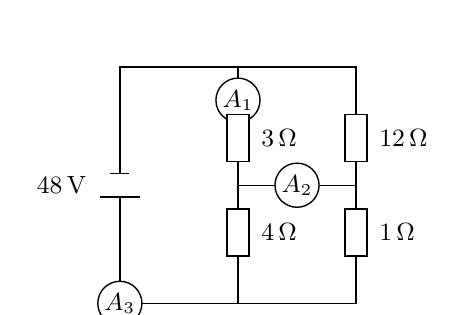
\begin{tikzpicture}[line width=0.5pt]
\draw (0,0)--(0,1.35); \draw (0,1.65)--(0,3)--(3,3)--(3,2.4); \draw (-0.25,1.35)--(0.25,1.35); \draw (-0.12,1.65)--(0.12,1.65);
\node[left] at (-0.3,1.5) {\small $48\,\mathrm{V}$};
\draw (1.5,3)--(1.5,2.72); \draw (1.5,2.44)--(1.5,2.4);
\draw (1.5,1.8)--(1.5,1.2); \draw (1.5,0.6)--(1.5,0)--(0.28,0); \draw (-0.28,0)--(0,0);
\draw (3,1.8)--(3,1.2); \draw (3,0.6)--(3,0)--(1.5,0);
\draw (1.5,1.5)--(1.97,1.5); \draw (2.53,1.5)--(3,1.5);
\draw[fill=white] (1.5,2.58) circle (0.28); \node at (1.5,2.58) {\small $A_1$};
\draw[fill=white] (1.3599999999999999,1.8) rectangle (1.6400000000000001,2.4); \node[right] at (1.67,2.1) {\small $3\,\Omega$};
\draw[fill=white] (1.3599999999999999,0.6000000000000001) rectangle (1.6400000000000001,1.2); \node[right] at (1.67,0.9) {\small $4\,\Omega$};
\draw[fill=white] (2.86,1.8) rectangle (3.14,2.4); \node[right] at (3.17,2.1) {\small $12\,\Omega$};
\draw[fill=white] (2.86,0.6000000000000001) rectangle (3.14,1.2); \node[right] at (3.17,0.9) {\small $1\,\Omega$};
\draw[fill=white] (2.25,1.5) circle (0.28); \node at (2.25,1.5) {\small $A_2$};
\draw[fill=white] (0.0,0.0) circle (0.28); \node at (0.0,0.0) {\small $A_3$};
\end{tikzpicture}\end{center}
\noindent\fbox{\begin{minipage}{0.64\linewidth}\vspace{4pt}\textbf{33.}\ $A_1$ ampermetrning körsatişini (A) aniqlang.\\[6pt]\textbf{34.}\ $A_2$ ampermetrning körsatişini (A) aniqlang.\\[6pt]\textbf{35.}\ $A_3$ ampermetrning körsatişini (A) aniqlang.\vspace{4pt}\end{minipage}\vrule\hspace{6pt}\begin{minipage}{0.28\linewidth}\vspace{4pt}A)\ 12\\B)\ 7,5\\C)\ 6\\D)\ 3\\E)\ 15\\F)\ 9\vspace{4pt}\end{minipage}}\par\vspace{14pt}
\Needspace{9\baselineskip}
\noindent\textbf{36.}\ Qirrasining uzunligi 2 cm bölgan kub şaklidagi 2 ta muz bölagi asosining yuzasi 50 cm$^2$ bölgan, 45,6 g suv quyilgan silindrik idişda taşlandi. $\rho_{muz}=900$ kg/m$^3$.\par\smallskip
\medskip\noindent\textbf{a)\ Muzlar erib ketgandan söng suyuqlikning idiş tubiga beradigan bosimini (Pa) toping.}\par
\noindent\textit{Javob}: a)\ \blank\par
\medskip\noindent\textbf{b)\ Muzlar erib ketgandan söng suyuqlikning idiş tubiga beradigan bosim kuçini (N) hisoblang.}\par
\noindent\textit{Javob}: b)\ \blank\par
\medskip\noindent\textbf{Diqqat!} Javoblaringizni javoblar varaqasiga köçirib yozing.\par\vspace{10pt}
\Needspace{9\baselineskip}
\noindent\textbf{37.}\ Silindrik idişga teng massali suv va kerosin quyildi. Suyuqliklar ustunining umumiy balandligi 27 cm ga teng. $\rho_{kerosin}=800$ kg/m$^3$.\par\smallskip
\medskip\noindent\textbf{a)\ Suv ustunining balandligini (cm) aniqlang.}\par
\noindent\textit{Javob}: a)\ \blank\par
\medskip\noindent\textbf{b)\ Idiş tubidan 8 cm balandlikdagi nuqtada suyuqliklarning hosil qilgan umumiy bosimini (Pa) toping.}\par
\noindent\textit{Javob}: b)\ \blank\par
\medskip\noindent\textbf{Diqqat!} Javoblaringizni javoblar varaqasiga köçirib yozing.\par\vspace{10pt}
\Needspace{9\baselineskip}
\noindent\textbf{38.}\ Uzunligi 12 m, qiyalik burçagi $37^\circ$ bölgan silliq qiya tekislik tepasidan 20 kg massali jism sirpanib tuşdi. $\sin37^\circ=0,6$, $\cos37^\circ=0,8$.\par\smallskip
\medskip\noindent\textbf{a)\ Jismning qiya tekislik etagidagi tezligini (m/s) toping.}\par
\noindent\textit{Javob}: a)\ \blank\par
\medskip\noindent\textbf{b)\ Bu jarayonda oğirlik kuçining bajargan işini (J) toping.}\par
\noindent\textit{Javob}: b)\ \blank\par
\medskip\noindent\textbf{Diqqat!} Javoblaringizni javoblar varaqasiga köçirib yozing.\par\vspace{10pt}
\Needspace{9\baselineskip}
\noindent\textbf{39.}\ Bir atomli ideal gazga 60 J issiqlik berib, hajmi izobarik ravişda 3 marta oşirildi.\par\smallskip
\medskip\noindent\textbf{a)\ Bunda gazning absolyut temperaturasi qanday özgaradi?}\par
\noindent\textit{Javob}: a)\ \blank\par
\medskip\noindent\textbf{b)\ Gazning bajargan işini (J) aniqlang.}\par
\noindent\textit{Javob}: b)\ \blank\par
\medskip\noindent\textbf{Diqqat!} Javoblaringizni javoblar varaqasiga köçirib yozing.\par\vspace{10pt}
\Needspace{9\baselineskip}
\noindent\textbf{40.}\ Issiqlik siğimi 500 J/K bölgan idişda 10 $^\circ$C temperaturali 5 $\ell$ suv bor. Idişga $-5\,^\circ$C temperaturali 1 kg muz taşlandi. $c_{suv}=4200$ J/(kg$\cdot$K), $c_{muz}=2100$ J/(kg$\cdot$K), $\lambda_{muz}=330$ kJ/kg.\par\smallskip
\medskip\noindent\textbf{a)\ Natijaviy temperaturani ($^\circ$C) toping.}\par
\noindent\textit{Javob}: a)\ \blank\par
\medskip\noindent\textbf{b)\ Muzning olgan issiqlik miqdorini (kJ) aniqlang.}\par
\noindent\textit{Javob}: b)\ \blank\par
\medskip\noindent\textbf{Diqqat!} Javoblaringizni javoblar varaqasiga köçirib yozing.\par\vspace{10pt}
\Needspace{9\baselineskip}
\noindent\textbf{41.}\ Proton induksiyasi $B$ bölgan magnit maydonga tik uçib kirdi va $r$ radiusli aylana böylab harakatlana boşladi. $m$ — zarraning massasi, $e$ — elementar zaryad.\par\smallskip
\medskip\noindent\textbf{a)\ Uning aylaniş çastotasini aniqlang.}\par
\noindent\textit{Javob}: a)\ \blank\par
\medskip\noindent\textbf{b)\ Protonning tezligini aniqlang.}\par
\noindent\textit{Javob}: b)\ \blank\par
\medskip\noindent\textbf{Diqqat!} Javoblaringizni javoblar varaqasiga köçirib yozing.\par\vspace{10pt}
\Needspace{9\baselineskip}
\noindent\textbf{42.}\ Maydon kuçlanganligi $E$ bölgan bir jinsli elektr maydonda harakatlanayotgan proton $l$ masofaga köçib, $A$ nuqtadan $B$ nuqtaga yetib bordi (rasmda $AD\perp \vec E$).\par\smallskip
\begin{center}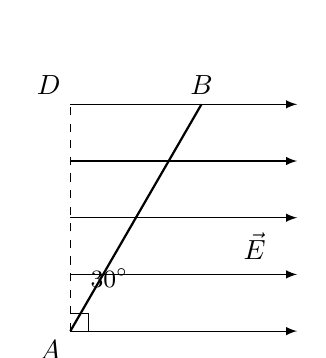
\begin{tikzpicture}[scale=0.9]\foreach \y in {0,0.8,1.6,2.4,3.2}{\draw[-latex] (0,\y)--(3.2,\y);}\draw (0.25,0)--(0.25,0.25)--(0,0.25);\draw[dashed] (0,0)--(0,3.2);\draw[thick] (0,0)--(1.85,3.2);\node[below left] at (0,0) {$A$};\node[above left] at (0,3.2) {$D$};\node[above] at (1.85,3.2) {$B$};\node at (2.6,1.2) {$\vec E$};\node at (0.55,0.75) {\small $30^\circ$};\end{tikzpicture}\end{center}
\medskip\noindent\textbf{a)\ Zarraning kinetik energiyasi qançaga özgarganini aniqlang.}\par
\noindent\textit{Javob}: a)\ \blank\par
\medskip\noindent\textbf{b)\ Zarra $ABDA$ yopiq yöl böylab köçirilganda elektr kuçlar bajaradigan işni aniqlang.}\par
\noindent\textit{Javob}: b)\ \blank\par
\medskip\noindent\textbf{Diqqat!} Javoblaringizni javoblar varaqasiga köçirib yozing.\par\vspace{10pt}
\Needspace{9\baselineskip}
\noindent\textbf{43.}\ Suvdagi nurning intensivligi 27 W/m$^2$ ga teng. $c=3\cdot10^8$ m/s.\par\smallskip
\medskip\noindent\textbf{a)\ Nurdagi elektromagnit maydon energiyasining ziçligini (J/m$^3$) aniqlang.}\par
\noindent\textit{Javob}: a)\ \blank\par
\medskip\noindent\textbf{b)\ Nur suvdagi közgudan tik akslansa, közguga beradigan bosimini (Pa) aniqlang.}\par
\noindent\textit{Javob}: b)\ \blank\par
\medskip\noindent\textbf{Diqqat!} Javoblaringizni javoblar varaqasiga köçirib yozing.\par\vspace{10pt}
\Needspace{9\baselineskip}
\noindent\textbf{44.}\ Quyoşning diametri $13,8\cdot10^{8}$ m ga, Yer bilan Quyoşn orasidagi masofa $1,5\cdot10^{11}$ m ga teng. Fokus masofasi 0,5 m bölgan Yerdagi linza ekranda Quyoşnning haqiqiy tasvirini hosil qilmoqda.\par\smallskip
\medskip\noindent\textbf{a)\ Tasvir bilan linza orasidagi masofani (mm) toping.}\par
\noindent\textit{Javob}: a)\ \blank\par
\medskip\noindent\textbf{b)\ Quyoşn tasvirining diametrini (mm) toping.}\par
\noindent\textit{Javob}: b)\ \blank\par
\medskip\noindent\textbf{Diqqat!} Javoblaringizni javoblar varaqasiga köçirib yozing.\par\vspace{10pt}
\Needspace{9\baselineskip}
\noindent\textbf{45.}\ Ğalayonlangan vodorod atomining ionlaşiş energiyasi 3,4 eV ga teng.\par\smallskip
\medskip\noindent\textbf{a)\ Atom fotonni yutib impuls momentini $2\hbar$ ga oşirsa, uning ionlaniş energiyasi (eV) nimaga teng bölişini aniqlang.}\par
\noindent\textit{Javob}: a)\ \blank\par
\medskip\noindent\textbf{b)\ Atom fotonni yutib impuls momentini $2\hbar$ ga oşirsa, undagi elektronning tezligi neça marta özgarişini aniqlang.}\par
\noindent\textit{Javob}: b)\ \blank\par
\medskip\noindent\textbf{Diqqat!} Javoblaringizni javoblar varaqasiga köçirib yozing.\par\vspace{10pt}
\end{document}